\begin{refsection}

\section{Introduction}

FRED-OX is a refactored version of the FRED fuel performance code, originally developed by Konstantin Mikityuk and collaborators for the analysis of MOX fuel behaviour in sodium-cooled fast reactors.

If FRED-OX is used in scientific publications, please cite the following references.

\begin{verbatim}
@article{Mikityuk2011FRED,
  author    = {Konstantin Mikityuk and Andrei Shestopalov},
  title     = {FRED fuel behaviour code: Main models and
               analysis of Halden IFA-503.2 tests},
  journal   = {Nuclear Engineering and Design},
  year      = {2011},
  volume    = {241},
  number    = {7},
  pages     = {2455--2461},
  doi       = {10.1016/j.nucengdes.2011.04.033}
}

@inproceedings{Kriventsev2015TopFuel,
  author    = {Vladimir Kriventsev and Andrei Rineiski and Werner Pfrang and
               Sara Perez-Martin and Konstantin Mikityuk and
               Grigori Khvostov},
  title     = {Benchmark on Behavior of MOX Fuel Pin Under
               Irradiation at Nominal Power in Sodium Fast Reactor},
  booktitle = {Proceedings of TopFuel 2015},
  year      = {2015},
  address   = {Zurich, Switzerland}
}
\end{verbatim}

\section{Base Irradiation Physics: MOX Fuel and Cladding (FRED-OX)}
\label{sec:fred_ox}

FRED-OX extends the FRED-ROD thermo-mechanical solver with irradiation physics relevant to mixed oxide (Pu-U-O) fuel. The following additional variables and phenomena are introduced:

\begin{itemize}
\item \textbf{Burnup} $B$ [MWd/kgU]: volumetric energy deposited in the fuel; drives all irradiation-dependent property changes.
\item \textbf{Fission gas generation and release} $\mu_{gen}$, $\mu_{rel}$ [mol]: produced xenon/krypton alter gap conductance and internal gas pressure.
\item \textbf{Fuel swelling} $\varepsilon^{sw}$ [-]: volumetric strain due to solid and gaseous fission products, reducing the gap width.
\item \textbf{Irradiation creep of cladding}: allows inelastic strain accumulation in austenitic cladding under irradiation (AIM1 steel).
\item \textbf{Burnup-dependent thermal conductivity} of MOX: phonon scattering by fission products degrades conductivity with burnup.
\item \textbf{Gas mixture conductance}: released Xe/Kr reduces the gap thermal conductance.
\end{itemize}

\subsection{MOX fuel thermal properties}
\label{sec:mox_correlations} For MOX fuel, the Philipponneau (1992) model is used for material thermal conductivity $k(T)$ \cite{philipponneau1992} and the  heat capacity from Popov et al. \cite{popov2000}. MATPRO correlations are used for the thermal expansion properties \cite{hagrman1981}. In the FRED-OX implementation, these MOX thermal-property correlations are implemented in \texttt{src/apps/fred\_ox/fuelpelletmaterial/FredOxMOX.cpp} (with the corresponding interface in \texttt{FredOxMOX.hpp}).

% -------------------------------------
\subsection{Burnup Evolution}
\label{sec:burnup}
% -------------------------------------

The local burnup per axial layer $j$ is tracked as an ordinary differential equation:

\begin{equation}
  \frac{dB_j}{dt} = \frac{q'''_j}{\rho_{f,0}}
  \label{eq:burnup_ode}
\end{equation}

where $q'''_j$ [W/m$^3$] is the local volumetric power density and $\rho_{f,0}$ [kg/m$^3$] the as-fabricated fuel density (the denominator converts from volumetric energy to specific energy).  The burnup stored in the DAE $y$-vector is scaled by $8.64\times10^{10}$ to convert from MWd/kgU to J/kgU for dimensional consistency with the SUNDIALS integrator.

% -------------------------------------
\subsection{Fission Gas Generation and Release (Waltar-Reynolds Model)}
\label{sec:fgr}
% -------------------------------------

\subsubsection{Fission Gas Generation}

Fission gas (predominantly Xe and Kr) is produced at a rate proportional to the fission rate.  The fission rate per unit volume is:

\begin{equation}
  \dot{F}_j = \frac{q'''_j}{210\,\text{MeV} \times 1.60214\times10^{-13}\,\text{J/MeV}}
  \quad \text{[fissions/(m}^3\text{s)]}
  \label{eq:fission_rate}
\end{equation}

With 25 gas atoms produced per 100 fissions (Waltar \& Reynolds \cite{waltar1981}), the global generation rate is:

\begin{equation}
  \frac{d\mu_{gen}}{dt}
  = \sum_j \frac{0.25\;\dot{F}_j\,V_j}{N_A}
  \quad \text{[mol/s]}
  \label{eq:fggen_ode}
\end{equation}

where $V_j = \pi(r_{fo}^2 - r_{fi}^2)\,\Delta z_j$ is the fuel volume of layer $j$ and $N_A = 6.022\times10^{23}$\,mol$^{-1}$.

\subsubsection{Fission Gas Release}

The Waltar-Reynolds model distinguishes three fuel zones based on temperature and burnup \cite{waltar1981}:

\begin{itemize}
\item \emph{Central restructured zone} ($T > 1773$\,K):
        \begin{equation}
          \text{FGR}_R = \max\!\left(0,\;
          1 - \frac{4.7}{B}\left(1 - e^{-B/5.9}\right)\right)
          \label{eq:fgr_restructured}
        \end{equation}
\item \emph{Unrestructured zone} ($B > 3.5$\,MWd/kgU): a burnup/power-threshold function gives partial release,
        \begin{equation}
          \mathrm{FGR}_U =
          \begin{cases}
            0, & B \le 3.5, \\
            \max\!\left(0,\,1-a_U\right), & B > 3.5,
          \end{cases}
        \end{equation}
with
        \begin{equation}
          a_U = \frac{25.6}{B-3.5}
                \left(1-e^{-(B/3.5-1)}\right)
                e^{-0.0125\,q_l},
        \end{equation}
where $q_l$ is the linear power density in kW/m. For $B\ge 49.2$\,MWd/kgU, an additional attenuation is applied, $a_U \leftarrow a_U\,e^{-0.3(B-49.2)}$.
\item \emph{As-fabricated zone}: FGR = 0.
\end{itemize}

Early in irradiation, the fuel pellet is relatively homogeneous. As power is applied, a strong radial temperature gradient develops:
\begin{equation}
  T_c \gg T_s,
\end{equation}
where $T_c$ is the centerline temperature and $T_s$ the fuel surface temperature. This drives thermal-gradient-driven pore migration from hot to cool regions and progressively restructures the pellet microstructure.

Over time, three distinct radial regions are observed and represented in the Waltar-Reynolds treatment:

\paragraph{Central Restructured Zone (CRSZ).} The CRSZ is the high-temperature inner region where the original fuel microstructure is replaced by large columnar grains.

\begin{itemize}
\item Very high temperature, typically above about $1800$--$2000^{\circ}$C.
\item Strong pore migration and redistribution of porosity.
\item Central void formation and grain coarsening (order of $10\,\mu$m to several hundred $\mu$m in representative micrographs).
\item Reduced grain-boundary area per unit volume.
\end{itemize}

In this region, the model assumes rapid gas release once restructuring is established, because pore connectivity increases and transport distances are shortened. Physically, the CRSZ is treated as a highly efficient gas-release region.

\paragraph{Unrestructured Zone.} The outer region remains below the restructuring threshold temperature and retains the original fabrication microstructure.

\begin{itemize}
\item Original equiaxed grains and porosity are largely preserved.
\item Gas remains trapped in grains and grain boundaries.
\item Release is diffusion-limited and evolves gradually with burnup.
\end{itemize}

Gas release in this region depends on temperature, burnup, diffusion coefficients, and grain size, so the Waltar-Reynolds framework treats it separately from the CRSZ.

\paragraph{As-fabricated outer zone.} At sufficiently low temperature and low local burnup, release is negligible in this simplified partition, so $\mathrm{FGR}=0$ for that outer zone.

The model therefore separates release into two active mechanisms:
\begin{itemize}
\item \emph{CRSZ contribution}: rapid release, often dominant at high power.
\item \emph{Unrestructured contribution}: diffusion-limited, slower release.
\end{itemize}

An illustrative decomposition is
\begin{equation}
  \mathrm{FGR} = \mathrm{FGR}_{\mathrm{CRSZ}} + \mathrm{FGR}_{\mathrm{unres}}.
  \label{eq:fgr_split}
\end{equation}

Figure~\ref{fig:waltar_reynolds_zones} shows an illustrative radial temperature profile, the three conceptual zones, and representative zone-wise FGR trends versus radius together with a typical radial burnup trend.

\begin{figure}[H]
  \centering
  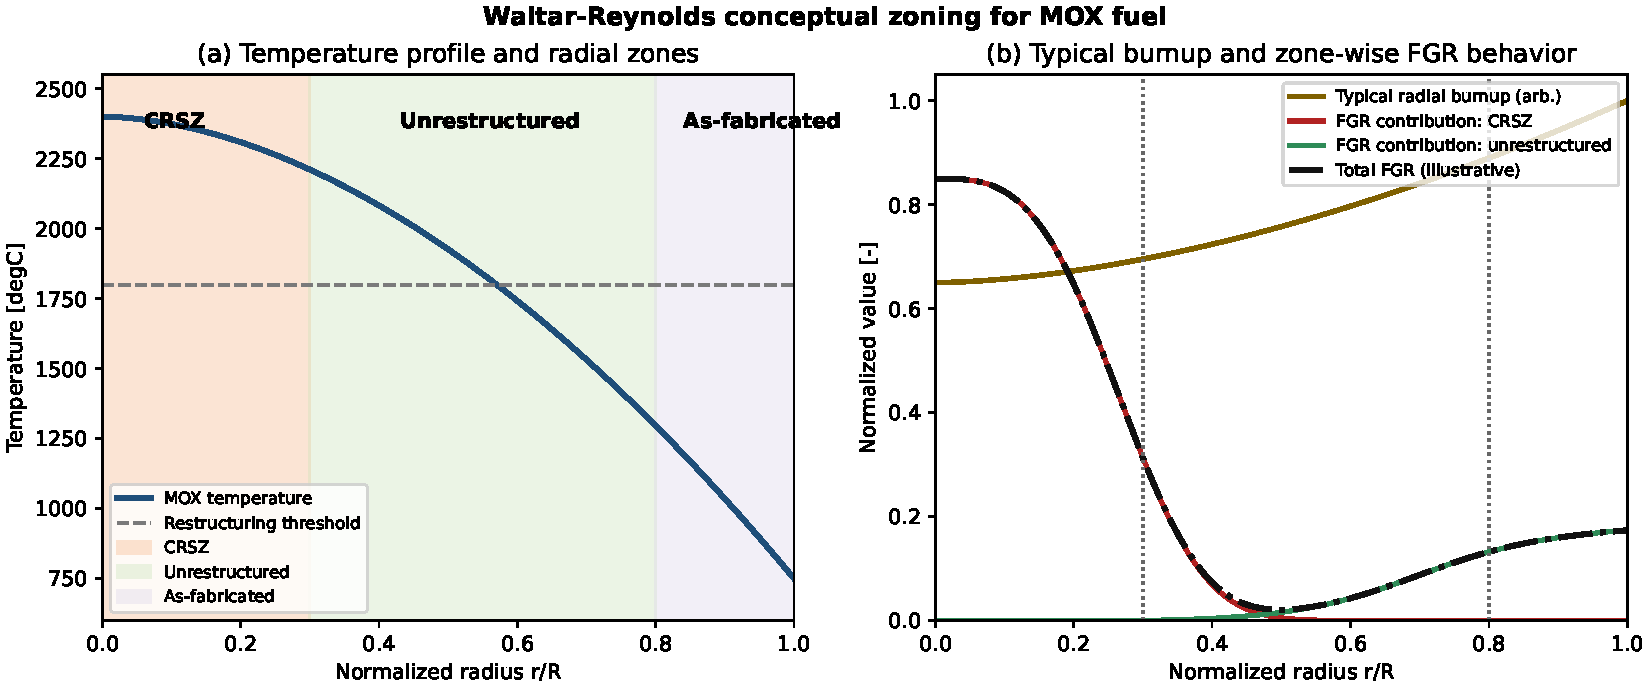
\includegraphics[width=0.98\textwidth]{images/waltar_reynolds_zones.pdf}
  \caption{Illustrative Waltar-Reynolds interpretation for MOX fuel: (a) a
  steep radial temperature profile and corresponding conceptual zone partition
  (CRSZ, unrestructured, and as-fabricated outer region); (b) representative
  zone-wise FGR behavior versus radius with a typical radial burnup profile.
  This figure is schematic and intended to clarify model logic, not to provide
  calibrated prediction data.}
  \label{fig:waltar_reynolds_zones}
\end{figure}

For each layer, the fractional area in each zone is evaluated from the radial temperature profile and the release fraction is area-averaged.  The global release ODE is:

\begin{equation}
  \frac{d\mu_{rel}}{dt}
  = \sum_j \frac{d\mu_{gen,j}}{dt} \cdot \overline{\text{FGR}}_j
  \label{eq:fgrel_ode}
\end{equation}

% -------------------------------------
\subsection{Internal Gas Pressure}
\label{sec:gpres}
% -------------------------------------

The internal gas pressure is determined by the ideal gas law applied to all void volumes:

\begin{equation}
  p_{gas} = \frac{(\mu_0 + \mu_{rel})\,R}{V_t}\times10^{-6}
  \quad \text{[MPa]}
  \label{eq:gpres}
\end{equation}

where $\mu_0$ [mol] is the initial fill-gas inventory, $R = 8.314$\,J/(mol\,K) is the universal gas constant, and the effective void volume at temperature is:

\begin{equation}
  V_t = \frac{V_{plenum}}{T_{pl}}
        + \sum_j \frac{\pi\,\Delta z_j\,(r_{ci,j}^2 - r_{fo,j}^2)}{T_{gap,j}}
        + \sum_j \frac{\pi\,\Delta z_j\,r_{fi,j}^2}{T_{ctr,j}}
  \label{eq:vt}
\end{equation}

with $T_{gap,j}$ the mean gas temperature in the gap of layer $j$, $T_{ctr,j}$ the central hole temperature, and $r_{fi,j}$, $r_{fo,j}$, $r_{ci,j}$ the deformed radii.

% -------------------------------------
\subsection{Gap Conductance with Fission Gas Mixture}
\label{sec:gap_ox}
% -------------------------------------

As fission gas is released into the plenum and gap, the gas mixture thermal conductivity decreases because Xe and Kr are poor thermal conductors.  Using a geometric-mean mixing rule:

\begin{equation}
  h_{gap}^{OX} = h_{medium}^{mix(He,Kr,Xe)} + h_{rad} + h_{contact}
  \label{eq:hgap_ox_modular}
\end{equation}

The medium term is computed with the Ross-Stoute / Lanning-Hann rarefied-gas temperature-jump model \cite{lanning1975}:

\begin{equation}
  h_{gas} = \frac{k_{gas}}{\delta_{eff} + g_{jump}}
  \label{eq:h_gas}
\end{equation}

\begin{equation}
  g_{jump} = \frac{0.024688\,k_{gas}\,\sqrt{T_{avg}}\cdot 2}{p\,\alpha}
  \label{eq:gjump}
\end{equation}

where $\delta_{eff} = \max(\delta, \delta_{rough})$ and $\delta_{rough}=\sqrt{\rho_f^2 + \rho_c^2}$, with $\alpha = \max(0.01,\;0.425 - 2.3\times10^{-4}T_{avg})$ (clamped to 1000 K). This keeps the thermal block modular while allowing FRED-OX-specific gas chemistry.

\begin{equation}
  k_{mix} = k_{He}^{x_{He}/\Sigma}
             \cdot k_{Kr}^{x_{Kr}/\Sigma}
             \cdot k_{Xe}^{x_{Xe}/\Sigma}
  \label{eq:kmix}
\end{equation}

where the mole fractions are computed from the fill gas ($\mu_0$\,mol He) and the released fission gas (composition: 88.46\% Xe, 7.69\% Kr, 3.85\% He by Waltar \& Reynolds \cite{waltar1981}).  Individual gas conductivities:

\begin{align}
  k_{He}(T) &= 2.639\times10^{-3}\,T^{0.7085} \label{eq:k_he2}\\
  k_{Kr}(T) &= 8.247\times10^{-5}\,T^{0.8363} \label{eq:k_kr}\\
  k_{Xe}(T) &= 4.351\times10^{-5}\,T^{0.8618} \label{eq:k_xe}
\end{align}

The additional terms are:

\begin{equation}
  h_{rad} = \sigma_{SB}\,f_\varepsilon\,(T_f^2 + T_c^2)(T_f + T_c)
  \label{eq:h_rad}
\end{equation}

\begin{equation}
  f_\varepsilon = \frac{1}{1/\varepsilon_f + (r_{fo}/r_{ci})(1/\varepsilon_c - 1)}
  \label{eq:frad}
\end{equation}

\begin{equation}
  h_{contact} = \frac{33.3\,k_m\,(p_{fc} - p_{gas})}{H_c\,\sqrt{\delta_{rough}}}
  \label{eq:h_contact}
\end{equation}

% -------------------------------------
\subsection{Fuel Swelling (MATPRO Model)}
\label{sec:swelling}
% -------------------------------------

The MATPRO fuel swelling model \cite{hagrman1981} distinguishes solid-fission- product swelling (independent of temperature) and gaseous-bubble swelling (strongly temperature-dependent):

\begin{align}
  \dot{\varepsilon}^{sw}_{solid}
    &= 2.5\times10^{-29}\,\dot{F}
    \label{eq:swel_solid}\\
  \dot{\varepsilon}^{sw}_{gas}
    &= 8.8\times10^{-56}\,(2800-T)^{11.73}\,
       e^{-0.0162(2800-T)}\,e^{-8\times10^{-27}\,E_{dep}}\,\dot{F}
    \quad (T < 2800\,\text{K})
  \label{eq:swel_gas}
\end{align}

where $\dot{F}$ [fissions/(m$^3$\,s)] is the local fission rate and $E_{dep} = B\,\rho_{f,0}$ [J/m$^3$] is the total deposited fission energy. The isotropic volumetric swelling strain is $\dot{\varepsilon}^{sw} = f_{mult}(\dot{\varepsilon}^{sw}_{solid} + \dot{\varepsilon}^{sw}_{gas})$, where $f_{mult}$ is a user-defined swelling multiplier.

The swelling strain enters the Hooke's law as an inelastic (eigenstrain) contribution in each direction:

\begin{align}
  E(\varepsilon_\theta - \varepsilon^{th} - \varepsilon^{sw}/3)
    &= \sigma_\theta - \nu(\sigma_r + \sigma_z) \\
  E(\varepsilon_r     - \varepsilon^{th} - \varepsilon^{sw}/3)
    &= \sigma_r     - \nu(\sigma_\theta + \sigma_z) \\
  E(\varepsilon_z     - \varepsilon^{th} - \varepsilon^{sw}/3)
    &= \sigma_z     - \nu(\sigma_\theta + \sigma_r)
\end{align}

% -------------------------------------
\subsection{MOX Thermal Conductivity (Philipponneau 1992)}
\label{sec:mox_k}
% -------------------------------------

The Philipponneau model \cite{philipponneau1992} gives the as-fabricated MOX conductivity and is extended in FRED-OX to include burnup degradation:

\begin{equation}
  k(T) = \left(\frac{1}{a_c + 2.493\times10^{-4}\,T}
               + 88.4\times10^{-12}\,T^3\right)
         \frac{1 - p}{1 + 2p}
  \label{eq:k_mox}
\end{equation}

where $p = 1 - \rho/\rho_{th}$ is the porosity and the stoichiometry- and burnup-dependent coefficient is:

\begin{equation}
  a_c = 1.320\sqrt{(2 - x) + 0.0093} - 0.091
        + \frac{0.0038\,B}{9.33}
  \label{eq:ac_burnup}
\end{equation}

with $x$ the oxygen-to-metal ratio deviation from stoichiometry and $B$ the burnup in MWd/kgU.

% -------------------------------------
\subsection{Cladding: AIM1 Steel with Irradiation Creep}
\label{sec:aim1}
% -------------------------------------

The AIM1 austenitic steel thermal conductivity and heat capacity are based on the legacy FRED correlations (also implemented in Luzzi \cite{luzzi2004}):

\begin{align}
  k_{AIM1}(T) &= 13.95 + 1.163\times10^{-2}(T - 273.15) \quad \text{[W/(m\,K)]} \\
  c_{p,AIM1}(T) &= 431.0 + 0.177\,T + 8.72\times10^{-5}\,T^2 \quad \text{[J/(kg\,K)]}
\end{align}

Irradiation creep of AIM1 is modelled through an empirical creep rate function $\dot{\varepsilon}^{cr} = f(\sigma, T, \dot{F})$.  T91 ferritic-martensitic steel (no irradiation creep in the current implementation) uses the corresponding implemented correlations for $k$, $c_p$, Young's modulus and thermal expansion.

\printbibliography[heading=subbibliography,title={References}]
\end{refsection}
